\documentclass[11pt]{article}

\usepackage[utf8]{inputenc}
\usepackage[T1]{fontenc}
\usepackage[margin=2.4cm]{geometry}
\usepackage{tikz}
\usepackage{graphicx}
\usepackage{float}
\usepackage{xcolor}
\usepackage{enumitem}
\usepackage{booktabs}
\usepackage{amsmath}
\usepackage{amssymb}
\usepackage{hyperref}
\usetikzlibrary{arrows.meta, positioning, fit, backgrounds, calc, decorations.pathreplacing}

\hypersetup{colorlinks=true, urlcolor=blue!60!black, linkcolor=black, citecolor=black}
\renewcommand{\figurename}{Figura}
\renewcommand{\tablename}{Tabla}

\definecolor{boxblue}{HTML}{2C5F8A}
\definecolor{boxgray}{HTML}{4A4A4A}
\definecolor{cellfill}{HTML}{EAF2FB}
\definecolor{cellc}{HTML}{FBE9D8}
\definecolor{good}{HTML}{2E7D32}
\definecolor{bad}{HTML}{C62828}

\tikzset{
  mod/.style={draw=boxblue, thick, rounded corners, fill=boxblue!8,
              align=center, inner sep=6pt, font=\small},
  big/.style={draw=boxblue, very thick, rounded corners, fill=boxblue!4,
              align=center, inner sep=8pt, font=\small},
  byte/.style={draw=boxgray, thick, minimum width=1.15cm, minimum height=0.9cm,
               fill=cellfill, font=\ttfamily\small},
  bytec/.style={draw=boxgray, thick, minimum width=1.15cm, minimum height=0.9cm,
               fill=cellc, font=\ttfamily\small},
  flow/.style={-{Stealth[length=2.5mm]}, thick, draw=boxgray},
  biflow/.style={{Stealth[length=2.5mm]}-{Stealth[length=2.5mm]}, thick, draw=boxgray},
}

\newcommand{\code}[1]{\texttt{#1}}

\title{\vspace{-1.2cm}\textbf{La extensión C (RVC) de RISC-V}\\[2pt]
\large Instrucciones comprimidas en un procesador segmentado}
\author{Steve Andy Ildefonso Santos}
\date{Arquitectura de Computadoras --- Proyecto 2 (material teórico)}

\begin{document}
\maketitle
\vspace{-0.7cm}

\begin{abstract}
\noindent
Este documento reúne la teoría necesaria para implementar la \textbf{extensión C}
(instrucciones comprimidas de 16 bits) de RISC-V sobre un procesador segmentado
de 5 etapas. Se parte de los conceptos previos (segmentación, contador de
programa, direccionamiento de memoria y \emph{little-endian}) y se construye hasta
el detalle de la solución: el \emph{fetch} con ventana deslizante, el incremento
variable del \code{PC}, el módulo descompresor, los formatos de codificación
comprimida y el repertorio concreto que implementaremos. El objetivo es que cada
decisión de diseño quede justificada, no memorizada.
\end{abstract}

\tableofcontents
\vspace{0.4cm}

%==================================================================
\section{Introducción y motivación}
%==================================================================

En sistemas embebidos y dispositivos con recursos limitados, el \textbf{tamaño
del código} es una restricción crítica: memorias pequeñas, cachés reducidas y
anchos de banda limitados hacen que cada byte cuente. Por eso RISC-V define la
\textbf{extensión ``C''} (\emph{compressed}, abreviada \textbf{RVC}): un conjunto
de instrucciones de \textbf{16 bits} que reemplazan a las instrucciones de 32
bits más comunes, reduciendo el tamaño del código típicamente entre un 25\,\% y un
30\,\% sin perder expresividad.

La clave que hace todo manejable es esta:
\begin{quote}
\itshape
Cada instrucción comprimida (16 bits) tiene \textbf{exactamente un equivalente}
de 32 bits al que puede expandirse.
\end{quote}
No necesitamos un procesador nuevo: necesitamos un \textbf{traductor} que
convierta los 16 bits a su forma de 32 bits \emph{antes} de que la instrucción
recorra el pipeline. Todo el reto se concentra entonces en una sola etapa
(\emph{Fetch}) y en un módulo nuevo (el \emph{descompresor}).

%==================================================================
\section{Conceptos previos}
%==================================================================

Antes de atacar RVC conviene tener firmes cuatro ideas: qué es un pipeline, qué
es el contador de programa, cómo se direcciona la memoria y qué significa
\emph{little-endian}.

%------------------------------------------------------------------
\subsection{El procesador segmentado (pipeline)}
%------------------------------------------------------------------

Un procesador segmentado divide el trabajo de cada instrucción en etapas, como
una línea de ensamblaje. Nuestro diseño usa \textbf{5 etapas}:

\begin{center}
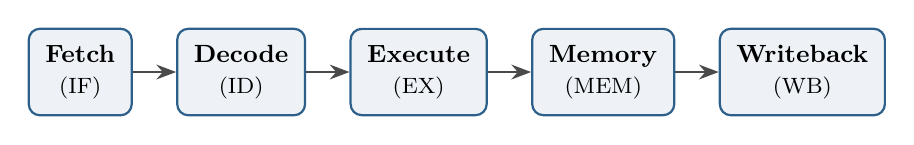
\begin{tikzpicture}[node distance=0.55cm]
  \node (f) [mod] {\textbf{Fetch}\\\footnotesize(IF)};
  \node (d) [mod, right=of f] {\textbf{Decode}\\\footnotesize(ID)};
  \node (e) [mod, right=of d] {\textbf{Execute}\\\footnotesize(EX)};
  \node (m) [mod, right=of e] {\textbf{Memory}\\\footnotesize(MEM)};
  \node (w) [mod, right=of m] {\textbf{Writeback}\\\footnotesize(WB)};
  \draw[flow] (f)--(d); \draw[flow] (d)--(e); \draw[flow] (e)--(m); \draw[flow] (m)--(w);
\end{tikzpicture}
\end{center}

\noindent
Cada etapa hace una parte del trabajo y pasa la instrucción a la siguiente:

\begin{center}
\begin{tabular}{@{}ll@{}}
\toprule
\textbf{Etapa} & \textbf{Qué hace} \\
\midrule
\textbf{Fetch}     & \textbf{lee} la instrucción de la memoria y decide la siguiente dirección \\
\textbf{Decode}    & interpreta los bits: qué instrucción es y qué registros usa \\
\textbf{Execute}   & \textbf{ejecuta} (la ALU suma, resta, compara, etc.) \\
\textbf{Memory}    & accede a la memoria de datos (\code{lw}/\code{sw}) \\
\textbf{Writeback} & guarda el resultado en el registro destino \\
\bottomrule
\end{tabular}
\end{center}

\noindent
En un ciclo de reloj hay \textbf{5 instrucciones distintas avanzando a la vez},
una en cada etapa. Un punto que será central para RVC:

\begin{quote}
\itshape
En \emph{Fetch} la instrucción \textbf{no se ejecuta}: solo se \textbf{lee}. La
ejecución (la suma, el AND\dots) ocurre tres etapas después, en \emph{Execute}.
\end{quote}

La Tabla~\ref{tab:flujo} ilustra el solapamiento. Observe que \code{addi} se
\emph{lee} en el ciclo~1 pero se \emph{ejecuta} en el ciclo~3.

\begin{table}[H]
\centering
\small
\begin{tabular}{@{}cccccc@{}}
\toprule
ciclo & Fetch & Decode & Execute & Memory & Writeback \\
\midrule
1 & \code{addi} &             &             &             &  \\
2 & \code{add}  & \code{addi} &             &             &  \\
3 & \code{sub}  & \code{add}  & \textbf{\code{addi}} &    &  \\
4 &             & \code{sub}  & \code{add}  & \code{addi} &  \\
5 &             &             & \code{sub}  & \code{add}  & \code{addi} \\
\bottomrule
\end{tabular}
\caption{Tres instrucciones avanzando por el pipeline. \code{addi} se lee en el
ciclo 1 y se ejecuta en el 3.}
\label{tab:flujo}
\end{table}

%------------------------------------------------------------------
\subsection{El contador de programa (PC)}
%------------------------------------------------------------------

El \textbf{PC} (\emph{Program Counter}) es un registro que guarda la
\textbf{dirección de la instrucción que toca leer ahora}. Cada ciclo, la etapa
Fetch hace dos cosas en paralelo con el PC:

\begin{enumerate}[noitemsep, leftmargin=1.6em]
  \item \textbf{Leer}: usa el PC como dirección para la memoria de instrucciones
        y obtiene la instrucción, que entra al pipeline.
  \item \textbf{Avanzar}: calcula la \textbf{siguiente} dirección
        (\code{PC + 4} en RISC-V base) y la deja lista para el próximo ciclo.
\end{enumerate}

\noindent
Ese ``\code{PC + algo}'' \textbf{no} ejecuta nada: solo prepara la dirección de
la próxima instrucción. Si hubo un salto tomado, la siguiente dirección no es
\code{PC+4} sino la \emph{dirección destino}, que decide la etapa Execute.

%------------------------------------------------------------------
\subsection{Direccionamiento de memoria: por byte y por palabra}
%------------------------------------------------------------------

La memoria se direcciona \textbf{por byte}: cada dirección apunta a un byte (8
bits). Pero físicamente nuestra memoria de instrucciones está organizada en
\textbf{palabras de 32 bits} (4 bytes). La palabra de índice $k$, que llamamos
\code{RAM[k]}, contiene los 4 bytes de las direcciones $4k,\,4k{+}1,\,4k{+}2,\,4k{+}3$.

Por eso, en RISC-V base, el PC avanza de \code{+4} en \code{+4}: cada instrucción
mide 4 bytes = una palabra. Para saltar a la siguiente palabra se suman 4
direcciones de byte.

\begin{center}
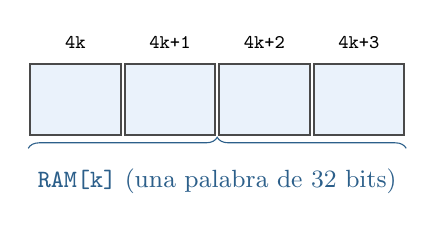
\begin{tikzpicture}
  \foreach \i/\lbl in {0/{4k},1/{4k+1},2/{4k+2},3/{4k+3}}{
    \node[byte] (b\i) at (\i*1.2,0) {};
    \node[font=\scriptsize\ttfamily] at (\i*1.2,0.72) {\lbl};
  }
  \draw[decorate, decoration={brace, amplitude=4pt}, boxblue]
        (-0.6,-0.62) -- (3*1.2+0.6,-0.62)
        node[midway, below=4pt, font=\small]{\code{RAM[k]} (una palabra de 32 bits)};
\end{tikzpicture}
\end{center}

%------------------------------------------------------------------
\subsection{Little-endian}
%------------------------------------------------------------------

\emph{Little-endian} define \textbf{cómo se ordenan los bytes} de un valor de
varios bytes dentro de la memoria: el byte de \textbf{dirección más baja} es el
\textbf{menos significativo}. Así, la palabra \code{RAM[k]} guarda:

\begin{center}
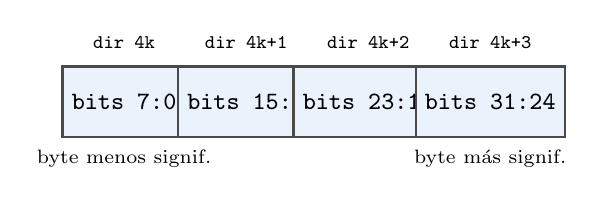
\begin{tikzpicture}
  \foreach \i/\lbl/\bits in {0/{4k}/{7:0},1/{4k+1}/{15:8},2/{4k+2}/{23:16},3/{4k+3}/{31:24}}{
    \node[byte, minimum width=1.5cm] (b\i) at (\i*1.55,0) {bits \bits};
    \node[font=\scriptsize\ttfamily] at (\i*1.55,0.75) {dir \lbl};
  }
  \node[font=\scriptsize] at (0,-0.72) {byte menos signif.};
  \node[font=\scriptsize] at (3*1.55,-0.72) {byte más signif.};
\end{tikzpicture}
\end{center}

\noindent
Importante: \emph{little-endian} \textbf{no} decide dónde puede caer el PC; solo
decide cómo se arma el \emph{valor} de la instrucción a partir de sus bytes. El
byte al que apunta el PC es siempre el \textbf{menos significativo} de la
instrucción, y de ahí se lee ``hacia adelante''.

%==================================================================
\section{La extensión C: idea general}
%==================================================================

RVC agrega instrucciones de \textbf{16 bits} que \textbf{conviven} con las de 32
en el mismo flujo de ejecución. No es un ``modo'' que se prende o apaga: se
pueden \textbf{mezclar} libremente.

\paragraph{Cómo se distingue una de otra.} Por los dos bits menos significativos
de la instrucción leída:
\begin{center}
\begin{tabular}{@{}ll@{}}
\toprule
\code{inst[1:0] == 2'b11} & instrucción de \textbf{32 bits} (normal) \\
\code{inst[1:0] != 2'b11} & instrucción de \textbf{16 bits} (comprimida, hay que expandir) \\
\bottomrule
\end{tabular}
\end{center}

\paragraph{La estrategia: descomprimir en Fetch.} El enunciado permite expandir
en Fetch o en Decode. Elegimos \textbf{Fetch} por una razón estratégica: si
expandimos los 16 bits a su forma de 32 bits \textbf{antes} de meter la
instrucción al registro de pipeline IF/ID, entonces

\begin{quote}\itshape
el resto del pipeline (Decode, Execute, Memory, Writeback, el control y la unidad
de riesgos) solo ve instrucciones RV32I normales y \textbf{no se entera} de que
existen las comprimidas.
\end{quote}

Esto convierte un problema que parece invasivo en uno \textbf{localizado en
Fetch}. La Figura~\ref{fig:fetch} muestra hacia dónde apuntamos.

\begin{figure}[H]
\centering
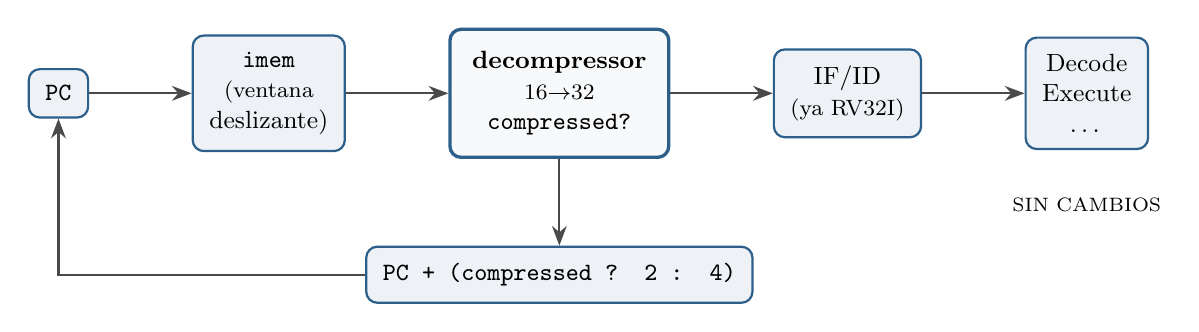
\begin{tikzpicture}[node distance=0.9cm and 1.3cm]
  \node (pc)   [mod] {\code{PC}};
  \node (imem) [mod, right=of pc] {\code{imem}\\\footnotesize(ventana\\deslizante)};
  \node (dec)  [big, right=of imem] {\textbf{decompressor}\\\footnotesize 16$\to$32\\\code{compressed?}};
  \node (ifid) [mod, right=of dec] {IF/ID\\\footnotesize(ya RV32I)};
  \node (rest) [mod, right=of ifid] {Decode\\Execute\\\dots};
  \draw[flow] (pc)--(imem); \draw[flow] (imem)--(dec); \draw[flow] (dec)--(ifid); \draw[flow] (ifid)--(rest);
  \node (inc) [below=1.1cm of dec, mod] {\code{PC + (compressed ? 2 : 4)}};
  \draw[flow] (dec) -- (inc);
  \draw[flow] (inc) -| (pc.south);
  \node[font=\scriptsize, align=center] at ($(rest.south)+(0,-0.7)$) {SIN CAMBIOS};
\end{tikzpicture}
\caption{Todo lo nuevo de RVC vive en \emph{Fetch}: leer (ventana deslizante),
medir ($+2/+4$) y traducir (descompresor). El resto del pipeline no cambia.}
\label{fig:fetch}
\end{figure}

%==================================================================
\section{El problema de la alineación}
%==================================================================

%------------------------------------------------------------------
\subsection{El PC ahora es par, pero no múltiplo de 4}
%------------------------------------------------------------------

Las instrucciones miden 2 o 4 bytes y siempre arrancan en una frontera de media
palabra (2 bytes). En consecuencia:

\begin{center}
\begin{tabular}{@{}ll@{}}
\toprule
\code{PC[0]} & \textbf{siempre 0} (el PC nunca es impar; no hay instrucciones de 1 byte) \\
\code{PC[1]} & \textbf{0 ó 1} (múltiplo de 4, o múltiplo de 4 más 2) \\
\bottomrule
\end{tabular}
\end{center}

\noindent
Que \code{PC[0]} sea siempre 0 está garantizado por construcción: el PC empieza
en 0, los incrementos son \code{+2} o \code{+4} (ambos pares), y los destinos de
salto se codifican en múltiplos de 2 (en \code{jalr} se fuerza con
\code{\{ALUResult[31:1], 1'b0\}}, que borra el bit 0). Dentro de una palabra, el
PC solo puede caer en el byte 0 o en el byte 2:

\begin{center}
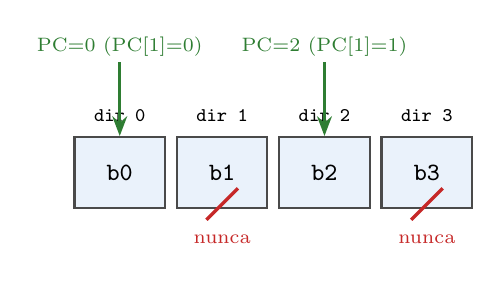
\begin{tikzpicture}
  \foreach \i/\lbl in {0/{0},1/{1},2/{2},3/{3}}{
    \node[byte] (b\i) at (\i*1.3,0) {b\i};
    \node[font=\scriptsize\ttfamily] at (\i*1.3,0.72) {dir \lbl};
  }
  \draw[flow, draw=good, very thick] (0,1.4) -- (b0.north);
  \draw[flow, draw=good, very thick] (2*1.3,1.4) -- (b2.north);
  \node[good, font=\scriptsize] at (0,1.6) {PC=0 (PC[1]=0)};
  \node[good, font=\scriptsize] at (2*1.3,1.6) {PC=2 (PC[1]=1)};
  \draw[draw=bad, very thick] (1*1.3-0.2,-0.6) -- (1*1.3+0.2,-0.2);
  \draw[draw=bad, very thick] (3*1.3-0.2,-0.6) -- (3*1.3+0.2,-0.2);
  \node[bad, font=\scriptsize] at (1.3,-0.85) {nunca};
  \node[bad, font=\scriptsize] at (3*1.3,-0.85) {nunca};
\end{tikzpicture}
\end{center}

\noindent
La consecuencia: si \code{PC[1]=1}, la instrucción empieza ``a la mitad'' de la
palabra. La memoria actual no sabe leer desde ahí.

%------------------------------------------------------------------
\subsection{Instrucciones a caballo entre dos palabras}
%------------------------------------------------------------------

Como las comprimidas miden 2 bytes, después de una de ellas la alineación se
corre, y una instrucción de \textbf{32 bits} puede quedar \textbf{partida entre
dos palabras de memoria}. Veámoslo con un programa mixto: una normal \code{A}
(32~bits), una comprimida \code{B} (16~bits) y otra normal \code{C} (32~bits).

\begin{figure}[H]
\centering
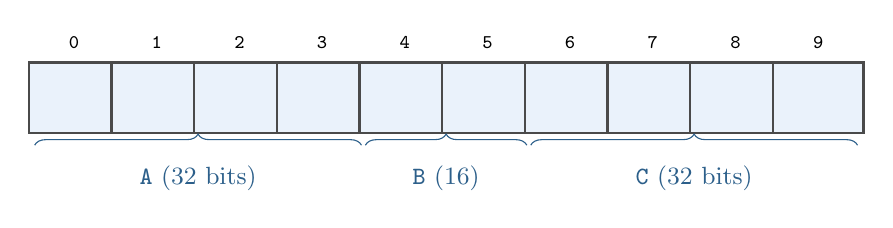
\begin{tikzpicture}
  \foreach \i in {0,...,9}{ \node[byte] (b\i) at (\i*1.05,0) {}; \node[font=\scriptsize\ttfamily] at (\i*1.05,0.7) {\i}; }
  \draw[decorate, decoration={brace, amplitude=4pt}, boxblue] (-0.5,-0.6) -- (3*1.05+0.5,-0.6) node[midway, below=4pt, font=\small]{\code{A} (32 bits)};
  \draw[decorate, decoration={brace, amplitude=4pt}, boxblue] (4*1.05-0.5,-0.6) -- (5*1.05+0.5,-0.6) node[midway, below=4pt, font=\small]{\code{B} (16)};
  \draw[decorate, decoration={brace, amplitude=4pt}, boxblue] (6*1.05-0.5,-0.6) -- (9*1.05+0.5,-0.6) node[midway, below=4pt, font=\small]{\code{C} (32 bits)};
\end{tikzpicture}
\caption{Disposición en memoria (flujo de bytes). \code{C} empieza en el byte 6.}
\label{fig:mixto}
\end{figure}

\noindent
Al empaquetar ese flujo en palabras de 32 bits (de a 4 bytes), las fronteras de
instrucción \emph{no} coinciden con las de palabra:

\begin{center}
\small
\begin{tabular}{@{}lll@{}}
\toprule
Palabra & Bytes & Contenido \\
\midrule
\code{RAM[0]} & 0,1,2,3 & \code{A} completa \\
\code{RAM[1]} & 4,5,6,7 & \code{B} (bytes 4,5) \;+\; \textbf{mitad baja de \code{C}} (bytes 6,7) \\
\code{RAM[2]} & 8,9,\dots & \textbf{mitad alta de \code{C}} (bytes 8,9) \;+\;\dots \\
\bottomrule
\end{tabular}
\end{center}

\noindent
\code{C} quedó partida: sus 16 bits bajos en \code{RAM[1][31:16]} y sus 16 altos
en \code{RAM[2][15:0]}. La memoria debe ser capaz de \textbf{reensamblarla}.

%==================================================================
\section{La solución: \emph{imem} con ventana deslizante}
%==================================================================

%------------------------------------------------------------------
\subsection{La idea}
%------------------------------------------------------------------

La restricción física es que la RAM solo se lee \textbf{por palabra entera}: no
existe ``dame los 32 bits que empiezan en el byte 6''. La solución es leer
\textbf{dos palabras consecutivas} ($\code{RAM[k]}$ y $\code{RAM[k+1]}$) y, según
\code{PC[1]}, recortar la ventana de 32 bits que empieza justo en el PC.

\begin{align*}
k    &= \code{PC[31:2]} \quad\text{(índice de palabra)}\\
w_0  &= \code{RAM[k]} \qquad\quad w_1 = \code{RAM[k+1]}\\[2pt]
\code{rd} &=
\begin{cases}
w_0 & \text{si } \code{PC[1]}=0 \quad\text{(alineado: la palabra entera sirve)}\\[2pt]
\{\,w_1[15{:}0],\; w_0[31{:}16]\,\} & \text{si } \code{PC[1]}=1 \quad\text{(cruza frontera)}
\end{cases}
\end{align*}

\paragraph{Punto clave.} La \code{imem} \textbf{siempre entrega 32 bits}, nunca
16. Es un ``tubo'' de ancho fijo. Cuando el PC apunta a una comprimida, igual
llegan 32 bits: los 16 bajos son la instrucción y los 16 altos son el comienzo de
la \emph{siguiente} (basura para este ciclo, que se descarta y se vuelve a leer
cuando el PC avance $+2$). Quién decide cuántos usar es el \emph{descompresor}, no
la memoria.

%------------------------------------------------------------------
\subsection{Por qué la combinación \texttt{\{w1[15:0], w0[31:16]\}}}
%------------------------------------------------------------------

Cuando \code{PC[1]=1} la instrucción empieza en el byte $4k{+}2$ y ocupa los
bytes $4k{+}2,\,4k{+}3,\,4k{+}4,\,4k{+}5$:

\begin{figure}[H]
\centering
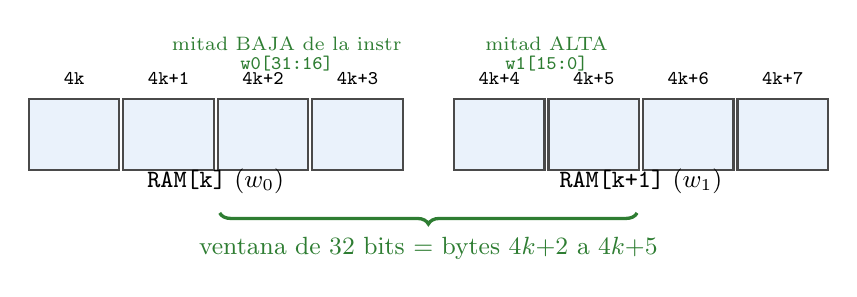
\begin{tikzpicture}
  \foreach \i/\lbl in {0/{4k},1/{4k+1},2/{4k+2},3/{4k+3}}{
    \node[byte] (a\i) at (\i*1.2,0) {}; \node[font=\scriptsize\ttfamily] at (\i*1.2,0.7) {\lbl};}
  \foreach \i/\lbl in {0/{4k+4},1/{4k+5},2/{4k+6},3/{4k+7}}{
    \node[byte] (c\i) at (\i*1.2+5.4,0) {}; \node[font=\scriptsize\ttfamily] at (\i*1.2+5.4,0.7) {\lbl};}
  \node[font=\small] at (1.8,-0.6) {\code{RAM[k]} ($w_0$)};
  \node[font=\small] at (1.8+5.4,-0.6) {\code{RAM[k+1]} ($w_1$)};
  \draw[decorate, decoration={brace, mirror, amplitude=4pt}, good, very thick]
        (2*1.2-0.55,-1.0) -- (5.4+1*1.2+0.55,-1.0)
        node[midway, below=5pt, font=\small, good]{ventana de 32 bits = bytes $4k{+}2$ a $4k{+}5$};
  \node[font=\scriptsize, good] at (2.7,1.15) {mitad BAJA de la instr};
  \node[font=\scriptsize, good] at (2.7,0.9) {\code{w0[31:16]}};
  \node[font=\scriptsize, good] at (5.4+0.6,1.15) {mitad ALTA};
  \node[font=\scriptsize, good] at (5.4+0.6,0.9) {\code{w1[15:0]}};
\end{tikzpicture}
\caption{Reensamblado: la mitad baja sale de la parte alta de $w_0$ y la mitad
alta de la parte baja de $w_1$. En Verilog \code{\{ALTO, BAJO\}}, de ahí
\code{\{w1[15:0], w0[31:16]\}}.}
\label{fig:ventana}
\end{figure}

%------------------------------------------------------------------
\subsection{El código}
%------------------------------------------------------------------

\begin{center}
\begin{minipage}{0.92\linewidth}
\begin{verbatim}
module imem(input  [31:0] a, output [31:0] rd);
  reg [31:0] RAM[63:0];
  wire [31:0] w0, w1;
  initial begin
    $readmemh("riscvtest.mem", RAM);
  end
  assign w0 = RAM[a[31:2]];
  assign w1 = RAM[a[31:2] + 1];
  assign rd = a[1] ? {w1[15:0], w0[31:16]} : w0;
endmodule
\end{verbatim}
\end{minipage}
\end{center}

\noindent
Las dos lecturas ($w_0$ y $w_1$) ocurren en paralelo (es hardware
combinacional); el mux con \code{a[1]} solo \emph{elige}.

%------------------------------------------------------------------
\subsection{Ejemplo a nivel de bits}
%------------------------------------------------------------------

Sea \code{RAM[k] = 0x11112222} y \code{RAM[k+1] = 0x33334444}.

\begin{center}
\begin{tabular}{@{}lll@{}}
\toprule
Caso & Cálculo & Resultado \code{rd} \\
\midrule
\code{PC[1]=0} & $w_0$ & \code{0x11112222} \\
\code{PC[1]=1} & $\{w_1[15{:}0],\, w_0[31{:}16]\} = \{\code{0x4444},\code{0x1111}\}$ & \code{0x44441111} \\
\bottomrule
\end{tabular}
\end{center}

\noindent
Para \code{PC[1]=1}, la instrucción \code{0x44441111} se armó con la parte alta de
\code{RAM[k]} (sus 16 bits bajos) y la parte baja de \code{RAM[k+1]} (sus 16
altos). Reensamblada correctamente.

\paragraph{Compatibilidad con RV32I.} Para un programa 100\,\% de 32 bits,
\code{PC[1]} es siempre 0, así que \code{rd = w0 = RAM[k]}: idéntico a la
\code{imem} original. Esa es la garantía de que los cimientos no rompen nada.

%==================================================================
\section{El incremento del PC: \texttt{+2} o \texttt{+4}}
%==================================================================

El incremento depende del \textbf{tamaño de la instrucción que se está leyendo
ahora}:
\[
\code{inc} = \code{compressed}\;?\;2 : 4,
\qquad
\code{PCPlusIncF} = \code{PCF} + \code{inc}.
\]

La señal \code{compressed} la produce el descompresor a partir de
\code{InstrF[1:0]}, en el mismo ciclo de Fetch. Renombramos \code{PCPlus4} a
\code{PCPlusInc} porque el valor ya no es siempre $+4$; además ese mismo valor
viaja por el pipeline como la \textbf{dirección de retorno} de \code{jal}/\code{jalr}
(para un \code{c.jal} debe ser \code{PC+2}). Los \textbf{saltos} siguen mandando:
el $+2/+4$ es solo el camino secuencial; si un branch o jump es tomado, el
próximo PC es la dirección destino.

\paragraph{Recorrido del PC (programa de la Figura~\ref{fig:mixto}).}
\begin{center}
\small
\begin{tabular}{@{}cccp{6.0cm}cc@{}}
\toprule
PC & \code{k} & \code{PC[1]} & ventana que arma \code{imem} & tipo & sig.\ PC \\
\midrule
0 & 0 & 0 & \code{RAM[0]} (\code{A} completa)                          & 32 bits ($+4$) & 4 \\
4 & 1 & 0 & \code{RAM[1]} $\to$ bits bajos = \code{B}                   & comprimida ($+2$) & 6 \\
6 & 1 & 1 & $\{$\code{RAM[2][15:0]}, \code{RAM[1][31:16]}$\}$ = \code{C} & 32 bits ($+4$) & 10 \\
\bottomrule
\end{tabular}
\end{center}

\noindent
En \code{PC=6} se ve la magia: tras la comprimida \code{B}, el PC quedó
desalineado (\code{PC[1]=1}) y la ventana deslizante reensambla \code{C} desde dos
palabras.

%==================================================================
\section{Resumen de la Fase 0 (``cimientos'')}
%==================================================================

La Fase 0 instala la infraestructura que necesita \emph{cualquier} comprimida,
sin implementar todavía ninguna instrucción concreta. Son tres cambios, cada uno
corrige una suposición de ``todo mide 32 bits'':

\begin{enumerate}[leftmargin=1.6em]
  \item \textbf{\code{imem} $\to$ ventana deslizante}: porque el PC puede caer a
        media palabra y una instrucción de 32 bits puede cruzar dos palabras.
  \item \textbf{Incremento \code{+2/+4}}: porque una comprimida mide 2 bytes.
  \item \textbf{\code{decompressor.v} (passthrough)}: el punto donde luego se
        expandirán los 16 bits; por ahora solo calcula \code{compressed} y deja
        pasar la instrucción.
\end{enumerate}

\noindent
\textbf{Propiedad de seguridad:} para programas RV32I puros nada cambia
(\code{PC[1]=0}, \code{compressed=0}), así que la regresión debe seguir pasando
igual que antes.

%==================================================================
\section{Formatos de codificación RVC}
%==================================================================

Toda comprimida son 16 bits. Dos campos orientan siempre: \code{inst[1:0]} (el
\emph{quadrant} u \code{op}: \code{00}=C0, \code{01}=C1, \code{10}=C2) y, en la
mayoría, \code{inst[15:13]} (\code{funct3}). Los cuatro formatos que usaremos:

\begin{center}
\small
\begin{tabular}{@{}llp{8.2cm}@{}}
\toprule
Formato & Campos principales & Uso \\
\midrule
\textbf{CR} & \code{funct4[15:12]}, \code{rd/rs1[11:7]}, \code{rs2[6:2]} & registros completos. \code{c.add} \\
\textbf{CI} & \code{funct3}, \code{imm[12]}, \code{rd/rs1[11:7]}, \code{imm[6:2]} & reg.\ completo + inmediato de 6 bits. \code{c.addi}, \code{c.lui}, \code{c.slli} \\
\textbf{CA} & \code{funct6[15:10]}, \code{rd'/rs1'[9:7]}, \code{funct2[6:5]}, \code{rs2'[4:2]} & registros restringidos. \code{c.sub/xor/or/and} \\
\textbf{CB} & \code{funct3}, \code{imm[12]}, \code{funct2[11:10]}, \code{rd'/rs1'[9:7]}, \code{imm[6:2]} & reg.\ restringido + inmediato. \code{c.srli/srai/andi} \\
\bottomrule
\end{tabular}
\end{center}

\noindent
\textbf{Lo cómodo de E2:} el inmediato \emph{no} está ``scrambleado''; es un bloque
contiguo de 6 bits $=\{\code{inst[12]}, \code{inst[6:2]}\}$. El reordenamiento
complejo de bits (offsets de memoria y de salto) aparece en la entrega
siguiente.

%==================================================================
\section{Registros restringidos \texorpdfstring{$rd'/rs2'$}{rd'/rs2'} (x8--x15)}
%==================================================================

En CA y CB los registros se codifican en \textbf{3 bits} y solo pueden ser
\textbf{x8 a x15} (los más usados). La conversión es directa: número real
$= 8 + \text{campo}$, es decir, anteponer \code{01} a los 3 bits.

\begin{center}
\small
\begin{tabular}{@{}ccl@{}}
\toprule
campo (3b) & registro real (5b) & nombre ABI \\
\midrule
\code{000} & \code{01000} = x8  & s0/fp \\
\code{001} & \code{01001} = x9  & s1 \\
\code{010} & \code{01010} = x10 & a0 \\
\code{011} & \code{01011} = x11 & a1 \\
\code{100} & \code{01100} = x12 & a2 \\
\code{101} & \code{01101} = x13 & a3 \\
\code{110} & \code{01110} = x14 & a4 \\
\code{111} & \code{01111} = x15 & a5 \\
\bottomrule
\end{tabular}
\end{center}

\noindent
En hardware: \code{reg\_real = \{2'b01, campo3\}}. En CI/CR el registro es de 5
bits completos (cualquiera de x0--x31) y no se aplica esta restricción.

%==================================================================
\section{Repertorio de la Entrega 2 (11 instrucciones)}
%==================================================================

Todas comparten la forma \code{rd = rd \emph{op} algo} (el destino es también el
primer operando: por eso RVC ahorra bits). Inmediato/shamt de 6 bits
$=\{\code{inst[12]}, \code{inst[6:2]}\}$.

\paragraph{Familia CI.}
\begin{center}
\small
\begin{tabular}{@{}lllll@{}}
\toprule
Instr & \code{op} & \code{funct3} & inmediato & Expande a \\
\midrule
\code{c.addi} & 01 & 000 & 6 bits con signo & \code{addi rd, rd, imm} \\
\code{c.lui}  & 01 & 011 & 6 bits $\to$ [17:12], con signo & \code{lui rd, imm} \\
\code{c.slli} & 10 & 000 & 6 bits = shamt (sin signo) & \code{slli rd, rd, shamt} \\
\bottomrule
\end{tabular}
\end{center}

\paragraph{Familia CR.}
\begin{center}
\small
\begin{tabular}{@{}llll@{}}
\toprule
Instr & \code{op} & \code{funct4} & Expande a \\
\midrule
\code{c.add} & 10 & 1001 & \code{add rd, rd, rs2} \quad(\code{rd},\code{rs2}$\neq$0) \\
\bottomrule
\end{tabular}
\end{center}

\paragraph{Familia CA (registros x8--x15, \code{funct6=100011}).}
\begin{center}
\small
\begin{tabular}{@{}llll@{}}
\toprule
Instr & \code{op} & \code{funct2 (inst[6:5])} & Expande a \\
\midrule
\code{c.sub} & 01 & 00 & \code{sub rd', rd', rs2'} \\
\code{c.xor} & 01 & 01 & \code{xor rd', rd', rs2'} \\
\code{c.or}  & 01 & 10 & \code{or  rd', rd', rs2'} \\
\code{c.and} & 01 & 11 & \code{and rd', rd', rs2'} \\
\bottomrule
\end{tabular}
\end{center}

\paragraph{Familia CB (\code{funct3=100}).}
\begin{center}
\small
\begin{tabular}{@{}llll@{}}
\toprule
Instr & \code{op} & \code{funct2 (inst[11:10])} & Expande a \\
\midrule
\code{c.srli} & 01 & 00 & \code{srli rd', rd', shamt} \\
\code{c.srai} & 01 & 01 & \code{srai rd', rd', shamt} \\
\code{c.andi} & 01 & 10 & \code{andi rd', rd', imm} (con signo) \\
\bottomrule
\end{tabular}
\end{center}

\paragraph{El despacho del descompresor.}
\begin{center}
\begin{minipage}{0.9\linewidth}
\begin{verbatim}
case (op = inst[1:0])
  01 (C1): segun funct3 = inst[15:13]:
             000 -> c.addi
             011 -> c.lui
             100 -> segun funct2 = inst[11:10]: 00 srli / 01 srai / 10 andi
             funct6=100011 -> segun funct2 = inst[6:5]: sub/xor/or/and
  10 (C2): segun funct3:
             000      -> c.slli
             funct4=1001 -> c.add
\end{verbatim}
\end{minipage}
\end{center}

%==================================================================
\section{Programas de prueba y verificación}
%==================================================================

Cada fase se valida con un programa que mezcle 16 y 32 bits y deje un resultado
comprobable en memoria. Ejemplo para \code{c.addi}:

\begin{center}
\begin{minipage}{0.7\linewidth}
\begin{verbatim}
addi x8, x0, 5    ; 32 bits  -> x8 = 5
c.addi x8, 3      ; 16 bits  -> x8 = 8
sw   x8, 0(x0)    ; Mem[0] = 8
\end{verbatim}
\end{minipage}
\end{center}

\paragraph{El cuidado más importante.} El ensamblador con \code{-march=rv32ic}
comprime \emph{automáticamente} lo que puede, y puede generar comprimidas que
\textbf{aún no implementamos} (\code{c.li}, \code{c.mv}\dots). Por eso, en cada
fase controlamos exactamente qué se comprime, con alguna de estas vías:
\begin{itemize}[noitemsep, leftmargin=1.6em]
  \item \code{.option norvc} / \code{.option rvc} alrededor de las líneas a comprimir;
  \item \code{.2byte 0x<encoding>} para emitir un código comprimido exacto a mano;
  \item escribir el \code{.mem} a mano en los primeros tests.
\end{itemize}

\paragraph{Oráculo de verificación.} Además de comprobar el valor en memoria,
mantener la \textbf{versión RV32I pura} del mismo programa y verificar que produce
un \textbf{estado de memoria idéntico} confirma que la expansión es correcta.

%==================================================================
\section{Fases de implementación (Entregas 2 y 3)}
%==================================================================

El trabajo se hace de forma \textbf{incremental}: cada fase compila, pasa sus
tests y genera su waveform antes de continuar. La división por fases sigue las
familias de codificación, de modo que cada una añade un bloque al \emph{case} del
descompresor sin rehacer lo anterior.

%------------------------------------------------------------------
\subsection{Entrega 2 --- instrucciones ALU/registro-inmediato}
%------------------------------------------------------------------

\begin{center}
\small
\begin{tabular}{@{}llp{7.6cm}@{}}
\toprule
Fase & Contenido & Notas \\
\midrule
\textbf{0} & Cimientos & \code{imem} ventana deslizante + \code{PCPlusInc} ($+2/+4$) + \code{decompressor.v} en \emph{passthrough}. La regresión RV32I debe seguir intacta. Es también el ``cambio extra al datapath'' que pide la rúbrica. \\
\textbf{E2.1} & \code{c.addi} (CI) & prueba de concepto: valida el camino completo \emph{fetch} desalineado $\to$ expandir $\to$ ejecutar. \\
\textbf{E2.2} & \code{c.lui}, \code{c.slli} (CI), \code{c.add} (CR) & registros completos; inmediato/shamt directos. \\
\textbf{E2.3} & \code{c.sub}, \code{c.and}, \code{c.or}, \code{c.xor} (CA) & introducen registros restringidos x8--x15. \\
\textbf{E2.4} & \code{c.srli}, \code{c.srai}, \code{c.andi} (CB) & registros restringidos + inmediato/shamt. \\
\textbf{E2.5} & Entrega & programa ISA mixto 16/32, waveforms por instrucción, sección del informe. \\
\bottomrule
\end{tabular}
\end{center}

\noindent
En toda la Entrega 2, como la expansión produce RV32I normal, \textbf{no se
modifican} \code{controller}, \code{aludec}, \code{extend} ni la unidad de
riesgos: todo el trabajo vive en \code{decompressor.v} y en los cimientos de la
Fase 0.

%------------------------------------------------------------------
\subsection{Entrega 3 --- memoria y control de flujo}
%------------------------------------------------------------------

La Entrega 3 cubre las 10 comprimidas restantes:
\code{c.lw}, \code{c.sw}, \code{c.lwsp}, \code{c.swsp}, \code{c.beqz},
\code{c.bnez}, \code{c.j}, \code{c.jal}, \code{c.jr}, \code{c.jalr}. Aquí aparece
la dificultad real que E2 no tenía:

\begin{itemize}[leftmargin=1.6em]
  \item \textbf{Inmediatos ``scrambleados''}: los formatos CL/CS (loads/stores),
        CB-branch (\code{c.beqz}/\code{c.bnez}) y CJ (\code{c.j}/\code{c.jal})
        reparten los bits del offset en posiciones \emph{no contiguas}. El
        descompresor debe \textbf{esparcir} esos bits a las posiciones exactas del
        inmediato I/S/B/J de RV32I para que el \code{extend} existente los
        reconstruya bien.
  \item \textbf{Offsets escalados}: \code{c.lw}/\code{c.sw} multiplican el offset
        por 4; \code{c.lwsp}/\code{c.swsp} son relativos a \code{x2} (\code{sp}).
  \item \textbf{Dirección de retorno \code{PC+2}}: \code{c.jal}/\code{c.jalr}
        deben enlazar con \code{PC+2}, lo que aprovecha el \code{PCPlusInc} que ya
        dejamos listo en la Fase 0.
\end{itemize}

\begin{center}
\small
\begin{tabular}{@{}llp{7.2cm}@{}}
\toprule
Fase & Contenido & Notas \\
\midrule
\textbf{E3.1} & \code{c.lw}, \code{c.sw} (CL/CS) & primer scrambling de inmediato (offset escalado $\times 4$). \\
\textbf{E3.2} & \code{c.lwsp}, \code{c.swsp} & relativos a \code{sp} (\code{x2}). \\
\textbf{E3.3} & \code{c.beqz}, \code{c.bnez} (CB-branch) & offset de salto con bits dispersos; expanden a \code{beq/bne rs1', x0, off}. \\
\textbf{E3.4} & \code{c.j}, \code{c.jal} (CJ), \code{c.jr}, \code{c.jalr} (CR) & saltos; \code{c.jal}/\code{c.jalr} enlazan con \code{PC+2}. \\
\textbf{E3.5} & Entrega & programa tipo algoritmo mixto, comparativa de tamaño y \emph{performance}, tabla de \emph{encoding} completa, informe. \\
\bottomrule
\end{tabular}
\end{center}

\paragraph{Sobre la unidad de riesgos.} Se revisa en cada fase, pero se espera que
\textbf{no requiera cambios}: sus comparaciones usan números de registro y son
agnósticas al ancho de la instrucción, ya que para cuando llegan a Decode todo es
RV32I expandido.

\paragraph{Sobre el \emph{performance}.} La descompresión es combinacional y no
añade etapas: el número de ciclos es el mismo. La ganancia es \textbf{tamaño de
código} ($\sim$25--30\,\%), no velocidad, en este modelo de memoria de un ciclo.

%==================================================================
\section*{Cierre}
\addcontentsline{toc}{section}{Cierre}
%==================================================================

En una frase: RVC se reduce a \textbf{enseñar a la etapa Fetch a leer y medir
instrucciones de 16 bits, y a traducirlas a RV32I antes de que entren al
pipeline}. La memoria con ventana deslizante resuelve la lectura desalineada; el
incremento $+2/+4$ resuelve el avance; el descompresor traduce. El resto del
procesador no se entera y no cambia. Implementar cada instrucción concreta es,
después de estos cimientos, solo rellenar el \emph{case} del descompresor según los
formatos y el repertorio aquí descritos.

\end{document}
